\documentclass[10pt]{article}
\usepackage[utf8]{inputenc}
\usepackage[T1]{fontenc}
\usepackage[margin=0.95in]{geometry}
\usepackage{amsmath,amssymb,amsthm}
\usepackage{booktabs}
\usepackage{array}
\usepackage{url}
\usepackage{microtype}
\usepackage{graphicx}
\usepackage{caption}
\usepackage{xcolor}
\usepackage[hidelinks]{hyperref}
\makeatletter\g@addto@macro{\UrlBreaks}{\do\_\do\.\do\/}\makeatother
\emergencystretch=3em
\tolerance=2000
% generated by gen_inputs.py from data/; do not edit
\newcommand{\BAMinHbar}{0.0877}
\newcommand{\BAMinHbarA}{0.5}
\newcommand{\BAHbarOne}{0.1238}
\newcommand{\BALamOne}{0.0942}
\newcommand{\BALamOneMargin}{0.0973}
\newcommand{\BAGammaStarOne}{0.313}
\newcommand{\BAGammaLamOne}{0.273}
\newcommand{\BACStaticOne}{0.11913}
\newcommand{\BACZpOne}{-0.96198}
\newcommand{\BARatioLo}{0.75}
\newcommand{\BARatioHi}{0.78}
\newcommand{\BAMarginShiftLo}{3}
\newcommand{\BAMarginShiftHi}{11}
\newcommand{\BBMinGammaStar}{0.2798}
\newcommand{\BBMinGammaStarA}{0.7}
\newcommand{\BBMinGammaLam}{0.245}
\newcommand{\BBInsideNarrow}{0.5, 0.6, 0.7, 0.8, 0.9, 1}
\newcommand{\BBInsideWide}{0.45, 0.5, 0.6, 0.7, 0.8, 0.9, 1, 1.1}
\newcommand{\BBSensLo}{0.81}
\newcommand{\BBSensHi}{1.21}
\newcommand{\BBCoulomb}{1.52}
\newcommand{\BBRatioOneNarrow}{1.41}
\newcommand{\BBRatioOneWide}{0.95}
\newcommand{\RayRatioOne}{-1.02}
\newcommand{\RayRatioHalf}{-1.01}
\newcommand{\RayRatioSeven}{-1.01}
\newcommand{\RayRatioEight}{-1.01}
\newcommand{\RayRatioTwelve}{-0.95}
\newcommand{\RaySlopeUpOne}{0.0711}
\newcommand{\RaySlopeArcOne}{-0.0695}
\newcommand{\SchaSpinHalf}{0.2745}
\newcommand{\SchaGammaHalf}{0.60}
\newcommand{\SchaBreakHalf}{0.617}
\newcommand{\SchaSpinSeven}{0.3076}
\newcommand{\SchaGammaSeven}{0.67}
\newcommand{\SchaBreakSeven}{0.518}
\newcommand{\SchaBreakOne}{0.427}
\newcommand{\SchaSpinThirteen}{0.2943}
\newcommand{\SchaGammaThirteen}{0.75}
\newcommand{\SchaBreakThirteen}{0.370}
\newcommand{\SchaOneLo}{0.300}
\newcommand{\SchaOneHi}{0.3347}
\newcommand{\SchaOneLapLo}{0.008}
\newcommand{\SchaOneLapFifteen}{0.117}
\newcommand{\HarmLapOneFifteen}{-0.101}
\newcommand{\HarmLapOneTen}{0.092}
\newcommand{\SchaMinDEOne}{\ensuremath{2.58\times10^{-5}}}
\newcommand{\SchaGammaAtLamOne}{0.287}
\newcommand{\SchaGammaFirstBelowOne}{0.87}
\newcommand{\SchaGammaLowAll}{0.60}
\newcommand{\SchaGammaHighAll}{0.75}
\newcommand{\ExtNPointsLo}{150}
\newcommand{\ExtStableLo}{144}
\newcommand{\ExtStableHi}{150}
\newcommand{\ExtUnstLo}{103}
\newcommand{\ExtUnstHi}{114}
\newcommand{\ExtBelow}{0}
\newcommand{\ExtMinDELo}{\ensuremath{1.2\times10^{-6}}}
\newcommand{\ExtMinDEHi}{\ensuremath{6.6\times10^{-6}}}
\newcommand{\ExtEdgeDELo}{\ensuremath{3.0\times10^{-4}}}
\newcommand{\ExtEdgeDEHi}{\ensuremath{1.7\times10^{-3}}}
\newcommand{\SlopeExtrap}{-3.843}
\newcommand{\SlopeHarm}{-3.848}
\newcommand{\SlopeFirst}{-3.807}
\newcommand{\SlopeLast}{-3.697}
\newcommand{\SlopeCoef}{14.7}
\newcommand{\FrozenMax}{\ensuremath{6.3\times10^{-6}}}
\newcommand{\FrozenBug}{0.52}
\newcommand{\FrozenN}{12}
\newcommand{\PimcDEInf}{\ensuremath{-2.86\times10^{-4}}}
\newcommand{\PimcShiftEight}{\ensuremath{-2.0\times10^{-4}}}
\newcommand{\PimcShiftTwelve}{\ensuremath{-2.0\times10^{-5}}}
\newcommand{\PimcNdEEight}{0.018}
\newcommand{\PimcNdETwelve}{0.041}
\newcommand{\PimcOmegaTwelve}{0.027}
\newcommand{\ShoulderMinRel}{-0.0448}
\newcommand{\ShoulderMinK}{4.82}
\newcommand{\ShoulderNegFrac}{44}
\newcommand{\GaussCtlErr}{\ensuremath{8.9\times10^{-16}}}
\newcommand{\ShoulderCutoffDiff}{\ensuremath{4.9\times10^{-11}}}
\newcommand{\RydEnergyHz}{100.7}
\newcommand{\RydRatio}{17.9}
\newcommand{\RydParam}{0.237}
\newcommand{\BAMarginEdgeLo}{\ensuremath{2.3\times10^{-5}}}
\newcommand{\BAMarginEdgeHi}{\ensuremath{2.4\times10^{-3}}}
\newcommand{\BATriMarginOne}{0.034}
\newcommand{\LadderJumpLo}{0.09}
\newcommand{\LadderJumpHi}{0.10}
\newcommand{\LadderDEAtHi}{\ensuremath{-2.86\times10^{-4}}}
\newcommand{\PimcDEs}{\ensuremath{4.68\times10^{-3}}}
\newcommand{\PimcDEzp}{-0.0496}
\newcommand{\HbarStarRangeLo}{0.088}
\newcommand{\HbarStarRangeHi}{0.178}
\newcommand{\LamOneRangeLo}{0.068}
\newcommand{\LamOneRangeHi}{0.131}
\newcommand{\ShoulderZero}{3.75}
\newcommand{\HbarStarNearRoot}{2.29}
\newcommand{\SchaHalfLapThree}{-0.013}
\newcommand{\SchaHalfLapFive}{0.003}
\newcommand{\CrossMax}{\ensuremath{8.9\times10^{-16}}}
\newcommand{\CrossN}{5}
\newcommand{\RustPassed}{63}
\newcommand{\RustFailed}{0}
\newcommand{\RustIgnored}{1}
\newcommand{\RootOne}{0.37668}
\newcommand{\RootTwo}{1.58148}

\newcommand{\tier}[1]{\textsf{[#1]}}
\newcommand{\sub}{\textsf{[sub]}}
\newcommand{\hb}{\hbar_{\mathrm{eff}}}
\newcommand{\Ezp}{E_{\mathrm{zp}}}
\newcommand{\Est}{E_{\mathrm{st}}}
\newcommand{\tr}{\operatorname{tr}}
\renewcommand{\Re}{\operatorname{Re}}
\newcommand{\Lap}{\Delta_{\!\mathrm{h}}}
\DeclareCaptionFont{small}{\small}
\captionsetup{font=small,labelfont=bf}
\makeatletter\newcommand{\tabinput}[1]{\@@input #1 }\makeatother

\title{\Large\bfseries The harmonic triangular-to-oblique instability of the quantum Gaussian-core crystal:\\
first order, near the Lindemann melting estimate,\\
and absent in the self-consistent harmonic approximation\\[3pt]
\normalsize\mdseries A preregistered negative result}
\author{Xavier Callens (SocrateAI Lab)}
\date{Preprint v1, 2026-10-26 (revised after an independent AI audit)}
\hypersetup{pdftitle={The harmonic triangular-to-oblique instability of the quantum Gaussian-core crystal: first order, near the Lindemann melting estimate, and absent in the self-consistent harmonic approximation -- a preregistered negative result},
  pdfauthor={Xavier Callens}}

\begin{document}
\maketitle
\begin{center}\small doi:10.5281/zenodo.23655625 \quad (not peer reviewed)\end{center}

\begin{center}\small Zenodo DOI to be assigned on release \quad (not peer reviewed; independent AI audit, no human audit)\end{center}

\noindent\textbf{AI-assistance disclosure.} This preprint, its Python and Rust code, its figures and its claim ledger were produced by AI agents
(Claude, Anthropic) under the author's direction. The author is responsible for the content. \emph{No human has audited the work.} A separate Claude agent, which wrote none of the code or text, audited it independently
(\texttt{AUDIT.md}, verdict \emph{ACCEPT\_WITH\_CORRECTIONS}, with its own from-scratch recomputation; Section~\ref{sec:audit}). Its four blocking and eleven nonblocking items are applied or answered in this revision (\texttt{REVISION.md}).
Producer, paper writer and the paper-stage reruns (Section~\ref{sec:rust}) belong to the same pipeline, so they are not producer~$\neq$~verifier checks; the auditor's recomputation is the verifier-separate check, and it is an AI check, not a human one. The numerical
results are Tier~X (floating point); none is machine-checked, and this paper contains no Lean statement.

\begin{abstract}
For the Gaussian-core pair potential $V=\varepsilon e^{-\pi a r^2/l^2}$ at one particle per site, the harmonic energy of a planar Bravais lattice of
shape $\tau$ is $E=\Est(\tau)+\hb\,\Ezp(\tau)$, with $\hb=\hbar/\sqrt{m\varepsilon l^2}$. We asked (preregistered, Proposal~2 item B1) whether
the triangular lattice then undergoes a quantum structural transition to a rhombic/oblique lattice, and whether it comes before melting and survives beyond the
harmonic approximation. The preregistered kill criterion reads, verbatim: \emph{``if the transition lies beyond melting or disappears beyond harmonic,
report that (negative result)''}. \textbf{The criterion is met; this is a negative result.}
\textbf{Tier X.} Within the harmonic theory the triangular lattice stops being a local minimum at $\hb^*(a)=-c_{\mathrm{st}}/c_{\mathrm{zp}}$ for $a\in(\RootOne,\RootTwo)$
(minimum $\BAMinHbar$ at $a=\BAMinHbarA$; $\BAHbarOne$ at $a=1$), and the transition is \emph{first order} in the sense that a finite-distortion, dynamically stable oblique lattice reaches the triangular energy
earlier, at $\Lambda_1\approx\BARatioLo$--$\BARatioHi\,\hb^*$ ($\BALamOne$ at $a=1$; the competitor sits on the harmonic stability edge and is not an interior local minimum); for $a=0.5$--$1$ the measured slopes at the triangular point on the two inequivalent mirror rays are equal and opposite (ratio $\RayRatioOne$ at $a=1$), as the cubic invariant allowed by the order-3 stabiliser predicts; the first-order claim itself rests on $\Lambda_1<\hb^*$. The harmonic Lindemann ratio at the spinodal is at least $\BBMinGammaStar$ for every $a$ tested,
i.e.\ at or beyond the top of the quantum-Monte-Carlo band $\gamma_c\in[0.23,0.28]$ (but below the harmonic value $0.30$ for $a=\BCBelowALo$--$\BCBelowAHi$); at $\Lambda_1$ it is $\BBMinGammaLam$--$\BAGammaLamOne$ for $a=0.5$--$1$ (inside the band, so the Lindemann test alone
does not exclude $\Lambda_1$ there) and larger elsewhere. Where $\Lambda_1$ lies inside the band the negative verdict on the first-order point rests on SCHA alone. The anharmonic test, within SCHA: in the $T=0$ self-consistent harmonic approximation (SCHA, two implementations agreeing to $\CrossMax$) the triangular
lattice stays a local minimum and the lowest stable sampled lattice up to $\hb\approx0.27$--$0.33$ (the SCHA spinodal, $a$-dependent), where the SCHA Lindemann ratio is $\SchaGammaLowAll$--$\SchaGammaFirstBelowOne$, far beyond any melting estimate; the transition disappears within SCHA.
\textbf{Caveats.} SCHA is a variational Gaussian theory that omits the second-order cubic $O(\hbar^2)$ term, and the stiffening it finds is itself of that order, so this holds \emph{within SCHA} and is not a statement of physical absence; path-integral Monte Carlo was \textbf{not run} (blocked, with numbers); only Bravais lattices were compared;
the harmonic $\Lambda_1$ winners sit on the harmonic stability edge. \textbf{Tier C (quotation-checked literature; no Tier L).} Rydberg dressing realises a soft shoulder whose Fourier transform is negative in places, not a Gaussian; a pure Gaussian has no negative Fourier component, and Prestipino et al.\ call it the marginal non-clustering case.
\textbf{Inference, not literature (Tier X):} that ordinary quantum melting preempts the harmonic transition rests only on our Lindemann numbers and SCHA, as qualified above. The earlier result that the triangular lattice is a local maximum of $\Ezp$ (doi:10.5281/zenodo.23653833) stands as a statement about the harmonic functional only. A new Rust SCHA module (rusty-SUNDIALS commit \texttt{9e85e15}) is part of the work.
\end{abstract}

\paragraph{Tiers.} \tier{A}: kernel-checked Lean (none here). \tier{L}: a theorem-like quotation passed by the Elenchus citation gate (none here, see Section~\ref{sec:lit}). \tier{C}: a human argument, a
definition, or a literature statement whose quotation was checked verbatim against the fetched source text (written \tier{C, quote}); statements taken from a sub-agent's reading and never re-read by us are written \sub{} and are in
no ledger row. \tier{X}: floating-point exploration, which never supports a claim by itself. Identifiers \texttt{B1-X-0001} refer to \texttt{ledger/ledger.json} (Section~\ref{sec:ledger}).

%=====================================================================
\section{Question, preregistration and what was deviated from}\label{sec:setting}
In the prior paper of this programme (P2, doi:10.5281/zenodo.23653833) the harmonic zero-point energy $\Ezp$ of a unit-covolume planar Bravais lattice was shown numerically \emph{not} to be minimised by the triangular
lattice for some completely monotone potentials; for the Gaussian the triangular lattice is a local \emph{maximum} of $\Ezp$ on $a\in(\RootOne,\RootTwo)$ \tier{X, from P2}. Since the static energy is minimised by the triangular lattice (Montgomery's theorem,
via P2), the total $\Est+\hb\Ezp$ must change its minimiser at some quantum parameter. B1 asks where, and whether it is physical.

\paragraph{Preregistered statements} (\texttt{results/proposal2/2026-10-26/preregistration.json}, item B1). B1a (X): $\hb^*(a)$ for $a\in(0.377,1.581)$. B1b: compare with a Lindemann melting estimate (harmonic $\langle u^2\rangle$).
B1c: anharmonic check (SCHA; path-integral Monte Carlo at a few points if feasible). B1d (L): relevance to Rydberg-dressed atoms from verified literature. Priors: B1a $0.85$, B1b (transition before melting) $0.4$, B1c (survives) $0.25$.
\textbf{Kill:} ``if the transition lies beyond melting or disappears beyond harmonic, report that (negative result)''.

\paragraph{Deviations and post hoc choices} (none changes a prior or the kill condition). (i) The first-order point $\Lambda_1$ and its sampled search (Section~\ref{sec:first}) are our definition, not preregistered. (ii) The Lindemann comparison band
$\gamma_c\in[0.23,0.28]$ (QMC true-$\langle u^2\rangle$ values) was chosen by the producer; we also show the harmonic value $0.30$ (Section~\ref{sec:lind}). (iii) The continuation-seeded SCHA run beyond the harmonic stability edge, the Rust SCHA module and the ray-slope test
were added to close gaps we found. (iv) PIMC was \emph{not run}: blocked (Section~\ref{sec:pimc}). (v) Only Bravais lattices with one particle per cell are compared. (vi) In B1d the sources we re-read are only four (Section~\ref{sec:lit}).

%=====================================================================
\section{Step-by-step human derivation}\label{sec:human}
\paragraph{Step 0: model and units \tier{C, B1-C-0001}.} Particles of mass $m$ on a planar Bravais lattice $L_\tau$ of shape $\tau=x+iy$ ($y>0$), basis $a_1=(1/\sqrt y,0)$, $a_2=(x/\sqrt y,\sqrt y)$, one particle per cell of area $l^2=1$.
Pair potential $V(r)=\varepsilon\,e^{-\pi a r^2/l^2}$ ($a>0$). Lengths in $l$, energies in $\varepsilon$: $H/\varepsilon=\sum_i\bigl(-\tfrac12\hb^2\nabla_i^2\bigr)+\sum_{i<j}\tilde V$, with $\hb=\hbar/\sqrt{m\varepsilon l^2}$
(the same $\hbar_{\rm eff}$ that appears in P2's functional). In the Gaussian-core-model units $V=\varepsilon e^{-r^2/\sigma^2}$ one has $\rho\sigma^2=1/(\pi a)$ and $\hbar/\sqrt{m\varepsilon\sigma^2}=\hb\sqrt{\pi a}$.

\paragraph{Step 1: the harmonic energy, $E=\Est+\hb\Ezp$ \tier{C, B1-C-0001}.} Expanding about the lattice sites, the dynamical matrix is
$D(\mathbf k)=\sum_{R\ne0}(1-\cos\mathbf k\!\cdot\!R)\,\mathrm{Hess}\,V(R)$, with $\mathrm{Hess}\,V(R)=(-2\pi a I+4\pi^2a^2RR^{\mathsf T})e^{-\pi a|R|^2}$, and each phonon has energy $\hb\sqrt{\lambda_j(D)}$. The ground-state energy per
particle is
\[E(\tau)=\Est(\tau)+\hb\,\Ezp(\tau),\qquad \Est=\tfrac12\sum_{R\ne0}e^{-\pi a|R|^2},\qquad \Ezp=\tfrac12\Bigl\langle\sqrt{\lambda_1(D)}+\sqrt{\lambda_2(D)}\Bigr\rangle_{\mathrm{BZ}}.\]
A shape is \emph{dynamically stable} if $D(\mathbf k)\succeq0$ for all $\mathbf k$. $\Est(\tau)$ is minimised at $\rho=e^{i\pi/3}$ for every $a$ (Montgomery's theorem, cited second-hand through P2; the original was not opened). This is a statement about shapes at fixed density; it does not include the
stress that holds a non-triangular lattice in shape (Section~\ref{sec:limits}).

\paragraph{Step 2: curvature at the triangular point \tier{C, B1-C-0002}.} $E$ depends on the lattice only up to rotation, hence $E(\gamma\tau)=E(\tau)$ for $\gamma\in SL_2(\mathbb Z)$. The map $\gamma(\tau)=(\tau-1)/\tau$ fixes $\rho$ and has derivative the
rotation by $-120^\circ$ there (this is machine-checked in P2, Lean statement \texttt{hasDerivAt\_gamma}; quoted as prior work, not re-proved here). A $C^2$ invariant function then has zero gradient at $\rho$ and a scalar Hessian (a symmetric $2\times2$ matrix commuting with a $120^\circ$
rotation is scalar, also checked in P2), so
\[E(\tau)-E(\rho)=c\,\frac{|\tau-\rho|^2}{y_\rho^2}+O(|\tau-\rho|^3),\qquad c=\tfrac14\Lap E(\rho),\quad \Lap=y^2(\partial_x^2+\partial_y^2).\]
Both $\Est$ and $\Ezp$ have this form, with $c_{\mathrm{st}}$ and $c_{\mathrm{zp}}$, so $c(\hb)=c_{\mathrm{st}}+\hb\,c_{\mathrm{zp}}$. The invariance, smoothness and chain-rule steps are not formalised.

\paragraph{Step 3: the harmonic spinodal \tier{C, B1-C-0002; numbers X, B1-X-0001}.} Montgomery gives $c_{\mathrm{st}}\ge0$ (a minimum; $c_{\mathrm{st}}>0$ is the computed value) and P2 found $c_{\mathrm{zp}}<0$ for $a\in(\RootOne,\RootTwo)$. Then $c(\hb)>0$ exactly when $\hb<\hb^*:=-c_{\mathrm{st}}/c_{\mathrm{zp}}$, and the
triangular lattice stops being a local minimum at $\hb^*$. If $c_{\mathrm{zp}}>0$ (outside the interval) there is no such $\hb^*$. The numbers $c_{\mathrm{st}}$ (exact pair sum of $h(u)=(u^2f')'$) and $c_{\mathrm{zp}}$ (Richardson stencil, Duffy--Gauss zone rule) are Tier~X.

\paragraph{Step 4: why the transition is first order \tier{C, B1-C-0003; test X, B1-X-0003}.} Use the disk coordinate $w=(\tau-\rho)/(\tau-\bar\rho)$, in which the order-3 stabiliser of $\rho$ acts as $w\mapsto\omega w$, $\omega=e^{2\pi i/3}$, and the
reflection $\tau\mapsto-\bar\tau$ composed with $\tau\mapsto\tau+1$ (every lattice energy is invariant under both) fixes $\rho$ and acts as a reflection of the $w$-plane; orient the axes so that it is $w\mapsto\bar w$. The stabiliser is thus $D_3$. A smooth function of $(w,\bar w)$ invariant under $D_3$ has Taylor expansion
in the invariants $|w|^2$, $\Re w^3$, $|w|^4,\dots$: the monomials $w^2$, $w\bar w^{\,2}$ etc.\ pick up a factor $\omega^{\pm1,\pm2}\neq1$ and are excluded, but $w^3+\bar w^3$ is allowed. With $w=re^{i\theta}$,
\[\Delta\Est=s_2r^2+s_3r^3\cos3\theta+O(r^4),\qquad \Delta\Ezp=z_2r^2+z_3r^3\cos3\theta+O(r^4),\qquad \hb^*=-s_2/z_2.\]
The \emph{tie coupling} $T(w)=\Delta\Est/(-\Delta\Ezp)$ is the value of $\hb$ at which the shape $w$ has the same energy as $\rho$ ($\Delta\Est>0$, $\Delta\Ezp<0$). Expanding,
\begin{equation}\label{eq:tie}T(w)=\hb^*+\kappa\,r\cos3\theta+O(r^2),\qquad \kappa=\frac{s_3+\hb^*z_3}{|z_2|}.\end{equation}
So if $\kappa\ne0$ a lower-energy shape exists for some $\hb<\hb^*$ on every circle around $\rho$ (on the rays with $\kappa\cos3\theta<0$): the triangular lattice is overtaken by a \emph{finite-distortion} state before its
quadratic coefficient vanishes, which is a first-order transition (a Landau cubic term). The six rays at $\theta=n\pi/3$ are the three mirror geodesics through $\rho$; adjacent rays have $\cos3\theta=\pm1$ alternately. The two
we scanned, $\Re\tau=\tfrac12$ upwards and $|\tau|=1$ towards $i$, differ by $60^\circ$, so (\ref{eq:tie}) predicts \emph{equal and opposite} slopes of $T$ in $|w|$. The symmetry argument is Tier~C; that $\kappa\ne0$ and the slope ratio are Tier~X (Section~\ref{sec:first}).

\paragraph{Step 5: the first-order point \tier{C, B1-C-0003; X}.} For a dynamically stable shape $\tau$ with $\Delta\Ezp<0$, $E(\tau)\le E(\rho)\iff\hb\ge T(\tau)$. Hence $\Lambda_1(a):=\min_{\tau\ \mathrm{stable}}T(\tau)$ is the smallest coupling at which a stable Bravais
competitor reaches the triangular energy. Because we minimise over a finite sample of the stable set, our $\Lambda_1$ is an upper bound on the true infimum; because stability is a closed condition, the infimum can sit on the stability boundary, and it does (Section~\ref{sec:first}).

\paragraph{Step 6: the Lindemann criterion and its $\gamma_c^2$ sensitivity \tier{C, B1-C-0004}.} At $T=0$ in the harmonic theory $\langle|u|^2\rangle/l^2=\hb\,U(a)$ with $U=\tfrac12\langle\tr D^{-1/2}\rangle_{\mathrm{BZ}}$ (both Cartesian components, finite
in 2D because the $1/|k|$ singularity is integrable). The Lindemann ratio is $\gamma=\sqrt{\langle|u|^2\rangle}/a_{nn}$ with $a_{nn}^2=2/\sqrt3$ for the unit-area triangular lattice. Setting $\gamma=\gamma_c$ gives the harmonic Lindemann coupling
\[\Lambda_L(\gamma_c)=\frac{\gamma_c^2a_{nn}^2}{U(a)}\qquad\Longrightarrow\qquad \frac{\Lambda_1}{\Lambda_L(\gamma_c)}=\Bigl(\frac{\gamma(\Lambda_1)}{\gamma_c}\Bigr)^2 .\]
Since $U$ is independent of $\hb$ at fixed $a$, $\Lambda_L\propto\gamma_c^2$: $\gamma_c\to0.9\gamma_c$ multiplies $\Lambda_L$ by $\BBSensLo$ and $\gamma_c\to1.1\gamma_c$ by $\BBSensHi$. This differs from the Coulomb Wigner crystal of the textbook of this programme
(doi:10.5281/zenodo.23295142, \tier{C}), where $\gamma^2\propto r_s^{-1/2}$ and hence $r_s^*\propto\gamma_c^{-4}$ ($0.9^{-4}=\BBCoulomb$). Lindemann is a rule of thumb, not a theorem; the value of $\gamma_c$ is the weakest input (Section~\ref{sec:lind}).

\paragraph{Step 7: the self-consistent harmonic approximation for Gaussians in closed form \tier{C, B1-C-0005}.} The trial state is the ground state of a harmonic crystal with an effective dynamical matrix $D_{\rm eff}(\mathbf k)$. The displacement difference $w_R=u_R-u_0$ is Gaussian with
covariance (mode sum of $\hbar/2\omega$ times $|e^{i\mathbf k\cdot R}-1|^2=2(1-\cos\mathbf k\!\cdot\!R)$)
\[C_R=\hb\,\bigl\langle(1-\cos\mathbf k\!\cdot\!R)\,D_{\rm eff}(\mathbf k)^{-1/2}\bigr\rangle_{\mathrm{BZ}}.\]
For the Gaussian potential every needed average is closed form. With $b=\pi a$, completing the square in $\int d^2w\,\mathcal N(w;0,C)\,e^{-b|R+w|^2}$ (precision $C^{-1}$ plus $2b I$) gives
\begin{equation}\label{eq:smooth}\langle V(R+w)\rangle=\det(I+2bC)^{-1/2}\exp\!\bigl(-b\,R^{\mathsf T}(I+2bC)^{-1}R\bigr),\end{equation}
and $\langle\mathrm{Hess}\,V(R+w)\rangle$ is the Hessian of the right side in $R$. The variational energy per particle is
\[E_{\rm SCHA}[D_{\rm eff}]=\tfrac{\hb}{4}\langle\tr D_{\rm eff}^{1/2}\rangle_{\mathrm{BZ}}+\tfrac12\sum_{R\ne0}\langle V(R+w_R)\rangle,\]
(the kinetic energy is half the harmonic zero-point energy of $D_{\rm eff}$), and it is stationary where $D_{\rm eff}(\mathbf k)=\sum_{R\ne0}(1-\cos\mathbf k\!\cdot\!R)\langle\mathrm{Hess}\,V(R+w_R)\rangle$ (the standard SCHA condition; we do not re-derive it but
verify it numerically, Section~\ref{sec:scha}), solved by mixing iteration. \emph{Small-$\hb$ limit:} $C_R=O(\hb)$ and $\langle V(R+w)\rangle=V(R)+\tfrac12\tr(C_R\,\mathrm{Hess}\,V(R))+O(C^2)$, so the potential term contributes a second $\tfrac{\hb}{4}\langle\tr D^{1/2}\rangle$
(since $\sum_R(1-\cos)\mathrm{Hess}\,V=D$): $E_{\rm SCHA}=\Est+\hb\Ezp+O(\hb^2)$. The $O(\hb^2)$ remainder is what SCHA treats only partially (Section~\ref{sec:limits}).

%=====================================================================
\section{Results}\label{sec:results}
\subsection{B1a: the harmonic spinodal $\hb^*(a)$ \tier{X, B1-X-0001}}\label{sec:spinodal}
\begin{table}[t]\centering\small\setlength{\tabcolsep}{4pt}
\caption{Harmonic results per $a$ (\texttt{data/result\_numbers.json}). $c_{\rm st}$, $c_{\rm zp}$: curvature coefficients at $\rho$; $\hb^*=-c_{\rm st}/c_{\rm zp}$; $\gamma$: harmonic Lindemann ratio
$\sqrt{\langle|u|^2\rangle}/a_{nn}$ at the triangular lattice; $\Lambda_1$ and its shape $\tau$: smallest tie coupling of a dynamically stable sampled lattice (Step~5). Tier~X.}\label{tab:main}
\begin{tabular}{rrrrrrrcr}\toprule
$a$ & $\rho\sigma^2$ & $c_{\rm st}$ & $c_{\rm zp}$ & $\hb^*$ & $\gamma(\hb^*)$ & $\Lambda_1$ & $\tau(\Lambda_1)$ & $\gamma(\Lambda_1)$\\\midrule
\tabinput{gen/tab_main.tex}
\bottomrule\end{tabular}\end{table}
The triangular lattice stops being a harmonic local minimum at $\hb^*(a)$ for every tested $a\in[0.4,1.5]$ (Table~\ref{tab:main}). $\hb^*$ has a minimum $\BAMinHbar$ at $a=\BAMinHbarA$ and diverges at both ends of $(\RootOne,\RootTwo)$ where $c_{\mathrm{zp}}\to0$.
Over $a\approx0.45$--$1.3$ it lies in $\HbarStarRangeLo$--$\HbarStarRangeHi$. Negative controls: $a=0.3$ and $a=2$ have $c_{\mathrm{zp}}>0$, hence no $\hb^*$, and no stable sampled shape has $\Delta\Ezp<0$ there; $a=0.378$ (just inside) gives $\hb^*=\HbarStarNearRoot$, consistent with the sign change at $\RootOne$.
\begin{figure}[t]\centering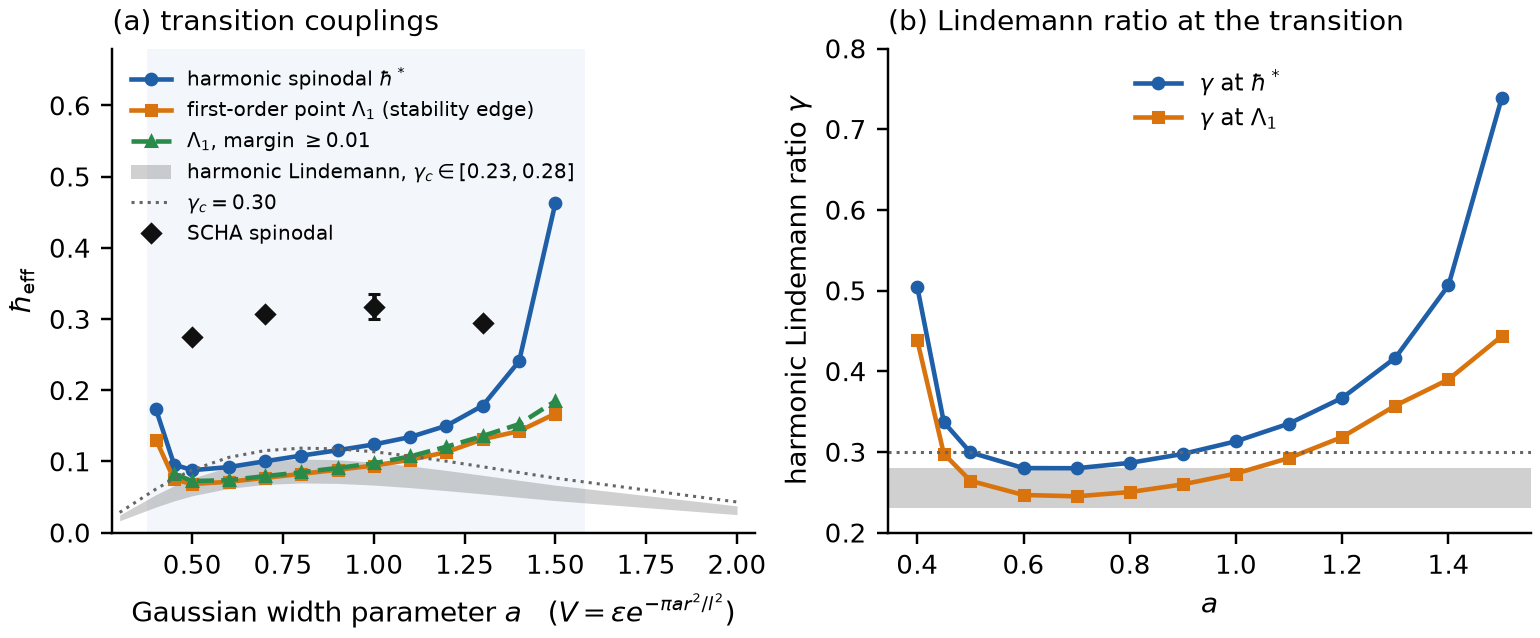
\includegraphics[width=\textwidth]{fig/fig_phase.png}
\caption{(a) Couplings $\hb^*$, $\Lambda_1$ (stability edge and margin $\ge0.01$), harmonic Lindemann coupling for $\gamma_c\in[0.23,0.28]$ (shaded) and $0.30$ (dotted), and SCHA spinodals (diamonds; at $a=1$ the interval $(\SchaOneLo,\SchaOneHi)$). (b) Harmonic Lindemann ratio at $\hb^*$ and at $\Lambda_1$. Tier~X.}\label{fig:phase}\end{figure}

\subsection{The transition is first order \tier{X, B1-X-0002, B1-X-0003}}\label{sec:first}
\emph{Meaning of ``first order''.} The competitor at $\Lambda_1$ is the minimiser of $E$ over the harmonically stable sampled set and it sits on that set's boundary; the producer records no interior minimum other than $\rho$ in the sampled stable set. So this is an energy crossing with a constrained finite-distortion competitor, not a crossing of two local minima: a finite-distortion stable lattice ties with $\rho$ before $c(\hb)$ vanishes.
At $a=1$ the lowest sampled stable competitor appears at $\Lambda_1=\BALamOne<\hb^*=\BAHbarOne$, so $\Lambda_1/\hb^*\in[\BARatioLo,\BARatioHi]$ for $a\in[0.45,1.2]$. Along the ladder in $\hb$ the argmin over the stable sample is the nearest neighbour of $\rho$ at
$\hb=\LadderJumpLo$ and jumps to the oblique lattice $0.30+0.96i$ at $\hb=\LadderJumpHi$ ($\Delta E=\LadderDEAtHi$ per particle there, from $\Delta\Est=\PimcDEs$ and $\Delta\Ezp=\PimcDEzp$), with no continuous growth of the distortion. The winner is oblique near $\tau\approx0.30+0.96i$ for
$0.45\le a\le1.2$ and near-centred-rectangular ($\Re\tau\approx\tfrac12$, $y\approx1.03$) for $a\ge1.3$ (Table~\ref{tab:main}).

\emph{The symmetry test.} Equation~(\ref{eq:tie}) predicts equal and opposite slopes of $T$ against $|w|$ on the rays $\Re\tau=\tfrac12$ and $|\tau|=1$. A quadratic fit over $0.003\le|w|\le0.035$ gives the slopes in Table~\ref{tab:rays}; the ratio is
$-1.0$ to within $2\%$ for $a=0.5$--$1$ (and $\RayRatioTwelve$ at $a=1.2$, where both signs are reversed). The opposite signs at the same $|w|$ are what a nonzero $D_3$-cubic term gives. Because the ray slopes change sign between $a=1$ and $a=1.2$, $\kappa$ must vanish somewhere in between (if the fits are accurate); there the local cubic argument is silent, yet $\Lambda_1/\hb^*$ stays at $\BARatioLo$--$\BARatioHi$, so what carries the first-order claim is the finite-distance competitor (Table~\ref{tab:main}), not the cubic term alone.
\begin{table}[t]\centering\small
\caption{Slope of the tie coupling against $|w|$ on the two mirror rays (quadratic fit, $|w|\le0.035$); prediction of Step~4: ratio $-1$.}\label{tab:rays}
\begin{tabular}{rrrr}\toprule $a$ & slope, $\Re\tau=\tfrac12$ & slope, $|\tau|=1$ & ratio\\\midrule\tabinput{gen/tab_rays.tex}\bottomrule\end{tabular}\end{table}
\begin{figure}[t]\centering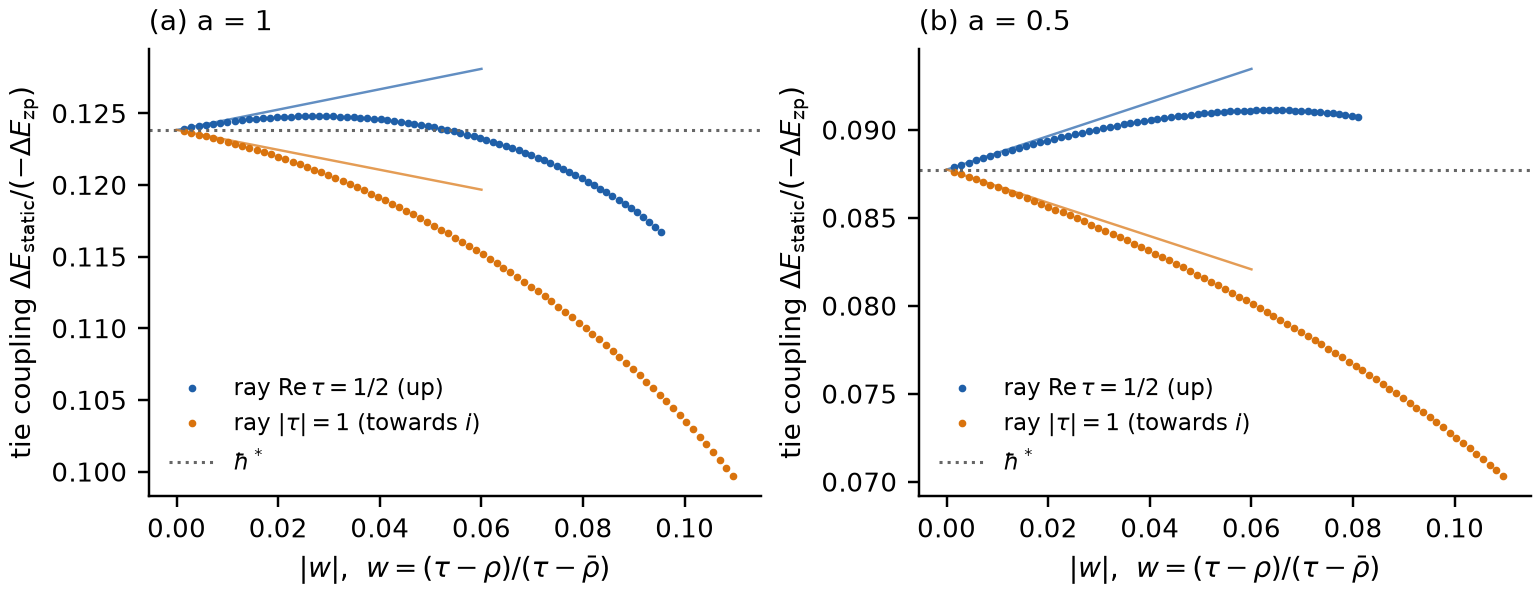
\includegraphics[width=0.92\textwidth]{fig/fig_rays.png}
\caption{Tie coupling $T$ against $|w|$ along the two mirror rays at $a=1$ and $a=0.5$; thin lines: linear parts of the quadratic fits; dotted: $\hb^*$. Tier~X.}\label{fig:rays}\end{figure}

\emph{The winners sit on the harmonic stability edge.} Their stability margin ($\min\lambda/|k|^2$) is $\BAMarginEdgeLo$ to $\BAMarginEdgeHi$, against $\BATriMarginOne$ for the triangular lattice at $a=1$. Restricting to shapes with margin $\ge0.01$ moves $\Lambda_1$
only by $\BAMarginShiftLo$--$\BAMarginShiftHi\,\%$ (at $a=1$: $\BALamOneMargin$), so ``first order with $\Lambda_1\ll\hb^*$'' is robust; but \emph{which} phase lies beyond is not determined by harmonic Bravais theory.

\subsection{B1b: Lindemann comparison \tier{X, B1-X-0004; $\gamma_c$ anchors C, quote}}\label{sec:lind}
The quantum-Monte-Carlo anchors for $\gamma_c$ in 2D boson crystals are, verbatim from Astrakharchik \emph{et al.}\ (cond-mat/0608246v2, p.~3, \tier{C, quote, B1-C-0101}): ``$\gamma=0.230(6)$'' for dipoles, ``$0.235(15)$ for Yukawa bosons'', ``$0.24(1)$ for Coulomb bosons'' and
``a hard-disks $\gamma=0.279$''. Their $\gamma$ is $\sqrt{\langle(r-r_c)^2\rangle}/a_L$ with $a_L$ ``the lattice length''; the same page defines the ``inverse lattice site length'' $a_L^{-1}=(\sqrt3 n/2)^{1/2}$, i.e.\ $a_L=a_{nn}$
(\tier{C, quote, B1-C-0116}); reading $\langle(r-r_c)^2\rangle$ as the total 2D displacement ($r$ is a 2D position) is
our reading (\tier{C, B1-C-0011}). (The first version of this paper wrongly said the definition was absent: the default text extraction scrambles that two-column sentence; \texttt{pdftotext -raw} recovers it.)
The harmonic value $\gamma=0.301$ at the Coulomb Wigner transition (textbook, \tier{C}) is a different quantity (harmonic, fermions). We therefore compare with the band $[0.23,0.28]$ and also show $0.30$ (Fig.~\ref{fig:phase}b, Table~\ref{tab:lind}).
\begin{table}[t]\centering\small\setlength{\tabcolsep}{4pt}
\caption{Harmonic Lindemann couplings $\Lambda_L(\gamma_c)$ and the ratio $\Lambda_1/\Lambda_L=(\gamma(\Lambda_1)/\gamma_c)^2$; ratios $<1$: the first-order point comes before melting. Tier~X.}\label{tab:lind}
\begin{tabular}{rrrrrrrr}\toprule $a$ & $\Lambda_L(0.23)$ & $\Lambda_L(0.28)$ & $\Lambda_L(0.30)$ & $\Lambda_1$ & $\Lambda_1/\Lambda_L(0.23)$ & $(0.28)$ & $(0.30)$\\\midrule\tabinput{gen/tab_lindemann.tex}\bottomrule\end{tabular}\end{table}
\textbf{Reading.} (a) At the \emph{spinodal} $\hb^*$ the ratio is $\ge\BBMinGammaStar$ for all $a$ (smallest at $a=\BBMinGammaStarA$, on the upper edge of the band, and rising towards both ends, Table~\ref{tab:main}): the spinodal is at or beyond melting for every $a$ if $\gamma_c\le0.28$ (at $a=\BBMinGammaStarA$ the margin is $\BBMinGammaStar$ against $0.28$, a tie to rounding); for $\gamma_c=0.30$ it precedes the Lindemann point for $a=\BCBelowALo$--$\BCBelowAHi$ ($\gamma(\hb^*)=\BCBelowLo$--$\BCBelowHi$). (b) At the first-order point
$\Lambda_1$ the ratio is never below $\BBMinGammaLam$, so $\Lambda_1>\Lambda_L(0.23)$ for every $a$ (melting first if $\gamma_c=0.23$); it is inside $[0.23,0.28]$ for $a=\BBInsideNarrow$ and inside $[0.23,0.30]$ for $a=\BBInsideWide$, i.e.\ $\Lambda_1\le\Lambda_L(\gamma_c)$ only for $\gamma_c\ge\gamma(\Lambda_1)$ (between $\BBMinGammaLam$ and $\BAGammaLamOne$ for $a=0.5$--$1$)
(at $a=1$: $\Lambda_1/\Lambda_L=\BBRatioOneNarrow$ for $\gamma_c=0.23$, $\BBRatioOneWide$ for $0.28$). With the $\gamma_c^2$ sensitivity of Step~6 ($\BBSensLo$--$\BBSensHi$ for $\pm10\%$) this is \emph{inconclusive to adverse}: B1b (prior $0.4$) is not supported, and the Lindemann argument alone does not close the case. (c) The anharmonic
$\langle u^2\rangle$ is larger: at $a=1$, $\Lambda_1=\BALamOne$ gives $\gamma_{\rm SCHA}=\SchaGammaAtLamOne$ against $\gamma_{\rm harm}=\BAGammaLamOne$, pushing towards ``melted first''. The QMC anchors are true-$\langle u^2\rangle$ values whereas $\gamma$ in Tables~\ref{tab:main}--\ref{tab:lind} is harmonic, so $\gamma_{\rm SCHA}$ is the closer like-for-like comparison: at $\hb^*$ it is $\ExtGamStarHalf$ ($a=0.5$) and $\ExtGamStarOne$ ($a=1$) (Table~\ref{tab:ext}), above the band top $0.28$ and, at $a=1$, above $0.30$.

\subsection{B1c: the transition does not survive the self-consistent harmonic approximation \tier{X, B1-X-0005, B1-X-0006}}\label{sec:scha}
The SCHA curvature is taken from the SCHA energy of each shape by a stencil, so the full second variation (including the bubble term) is included. Table~\ref{tab:scha} and Fig.~\ref{fig:scha}a show $\Delta E_{\rm SCHA}(\rho)\equiv\Lap E_{\rm SCHA}$ (positive: local minimum).
At $a=1$ and $\hb=0.15$, $\Lap E_{\rm SCHA}=\SchaOneLapFifteen$ where the harmonic value is $\HarmLapOneFifteen$; at $\hb=\SchaOneLo$ it is still $+\SchaOneLapLo$. The SCHA spinodal is $\SchaSpinHalf$ ($a=0.5$), $\SchaSpinSeven$ ($a=0.7$), $\SchaSpinThirteen$ ($a=1.3$) and in
$(\SchaOneLo,\SchaOneHi)$ at $a=1$, with SCHA Lindemann ratio $\SchaGammaLowAll$--$\SchaGammaFirstBelowOne$ (e.g.\ $\SchaGammaHalf$ at $a=0.5$, $\SchaGammaThirteen$ at $a=1.3$), more than twice $\gamma_c$. Near the SCHA breakdown no claim is made: at $a=1$ the sign of $\Delta E$ fluctuates between neighbouring couplings above $\hb\approx0.33$; at $a=0.5$, $\Lap E_{\rm SCHA}(\rho)$ is $\SchaHalfLapThree$ at $\hb=0.3$ but $\SchaHalfLapFive$ at $0.5$ (an apparent re-entrance); the iteration at $\rho$ breaks down at $\hb=\SchaBreakHalf,\SchaBreakSeven,\SchaBreakOne,\SchaBreakThirteen$ for $a=0.5,0.7,1,1.3$, and there $\gamma_{\rm SCHA}>0.6$ is outside any crystal description.
\begin{table}[t]\centering\scriptsize\setlength{\tabcolsep}{2.6pt}
\caption{SCHA results. Columns 4--8: $\Lap E_{\rm SCHA}(\rho)$ at $\hb=0.05,0.10,0.15,0.20,0.30$; col.~9: harmonic $\Lap E(\rho)=4(c_{\rm st}+\hb c_{\rm zp})$ at $\hb=0.10$; col.~10--11: SCHA spinodal (first sampled coupling with a stable competitor below $\rho$, or interval at $a=1$) and its $\gamma_{\rm SCHA}$;
col.~12--13: $\gamma_{\rm SCHA}$ at the harmonic $\Lambda_1$ and the smallest $\Delta E$ (competitor $-\rho$, per particle) among stable sampled shapes there ($>0$: triangular lowest). Tier~X.}\label{tab:scha}
\begin{tabular}{rrrrrrrrrrrrr}\toprule $a$ & $\hb^*$ & $\Lambda_1$ & .05 & .10 & .15 & .20 & .30 & harm.\ .10 & SCHA spin. & $\gamma$ & $\gamma(\Lambda_1)$ & $\min\Delta E$\\\midrule\tabinput{gen/tab_scha.tex}\bottomrule\end{tabular}\end{table}
\begin{figure}[t]\centering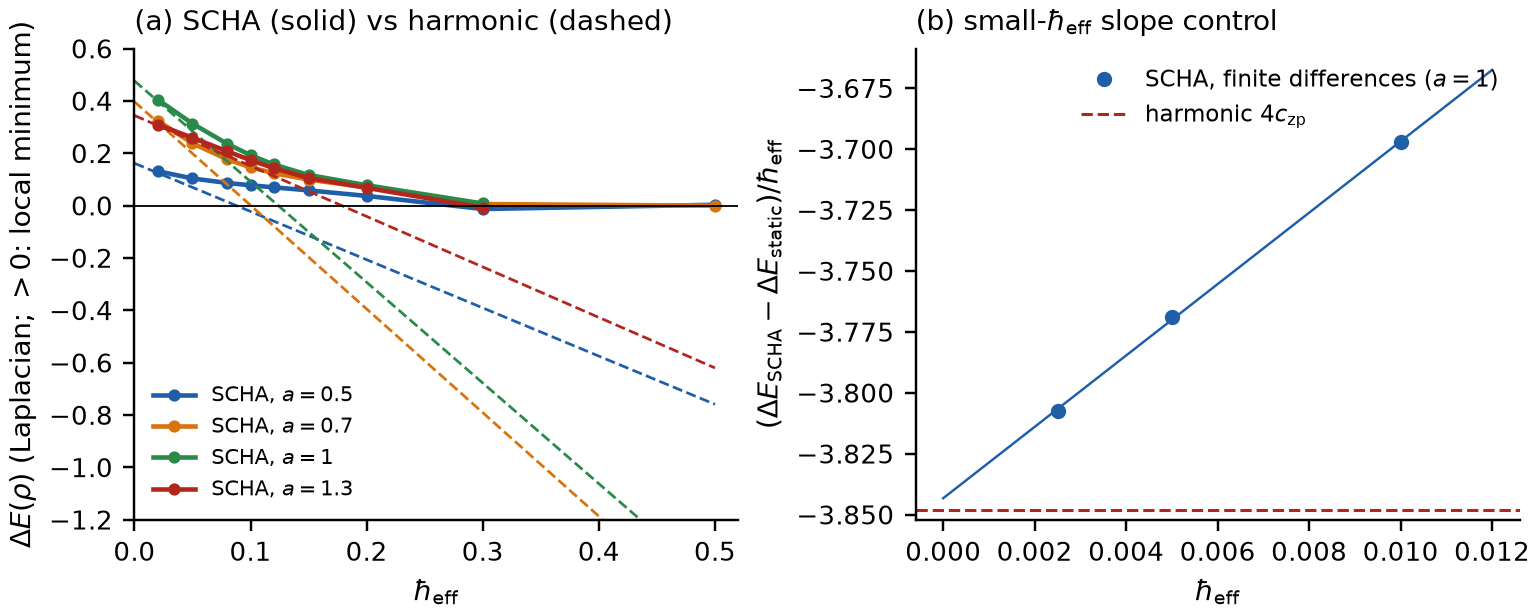
\includegraphics[width=\textwidth]{fig/fig_scha.png}
\caption{(a) $\Lap E(\rho)$ against $\hb$: SCHA (solid) and harmonic (dashed). (b) Small-$\hb$ slope control at $a=1$: $(\Lap E_{\rm SCHA}-\Lap E_{\rm st})/\hb$ tends to the harmonic $4c_{\rm zp}$. Tier~X.}\label{fig:scha}\end{figure}
\textbf{Competitors.} At the harmonic $\Lambda_1$ every sampled stable competitor (the arc and ray paths to $r=0.22$ and the harmonic edge winners) lies \emph{above} the triangular lattice in SCHA, by $\ge10^{-5}$ (last column; this minimum is set by the sampled point nearest $\rho$, i.e.\ by the local curvature). The harmonic edge winners lie higher: $\SchaEdgeWinOne$ above triangular at $a=1$ (winner $0.30+0.96i$; smallest over the edge points $\SchaEdgeMinOne$) and $\ge\SchaEdgeMinHalf$ at $a=0.5$ (the tabulated winner $(0.305,0.955)$ is $\SchaEdgeWinHalf$ above). A stable competitor below the triangular lattice first appears at the SCHA spinodal itself.
\textbf{Beyond the harmonic stability edge.} The plain solve is seeded from the bare $D$ and so rejects every harmonically unstable shape by construction. A continuation run seeds each shape with the converged $D_{\rm eff}$ of its neighbour, over 150 shapes per case (the arc $|\tau|=1$ from $\rho$ to $i$, $\Re\tau=\tfrac12$ up to $y=1.30$, and a strip $x\in[0.15,0.30]$ up to $y=1.12$),
at $a=1$ and $0.5$ and $\hb=\Lambda_1,\hb^*,0.2$ (Table~\ref{tab:ext}): $\ExtStableLo$--$\ExtStableHi$ are SCHA-stable, of which $\ExtUnstLo$--$\ExtUnstHi$ are harmonically unstable (anharmonicity stabilises them), and \textbf{none} lies below the triangular lattice. The lowest
competitor is the arc point nearest $\rho$ ($\ExtMinDELo$ to $\ExtMinDEHi$ above); the lowest shape beyond the harmonic edge is $\ExtEdgeDELo$ to $\ExtEdgeDEHi$ above.
\begin{table}[t]\centering\small\setlength{\tabcolsep}{4pt}
\caption{Continuation-seeded SCHA beyond the harmonic stability edge. $n$: shapes; stable: SCHA-stable; unst.: of these, harmonically unstable; below: SCHA-stable shapes below the triangular energy; min $\Delta E$: smallest over all, and over shapes beyond the harmonic edge. Tier~X.}\label{tab:ext}
\begin{tabular}{rrrrrrrrr}\toprule $a$ & $\hb$ & $\gamma_{\rm SCHA}(\rho)$ & $n$ & stable & unst. & below & min $\Delta E$ & beyond edge\\\midrule\tabinput{gen/tab_ext.tex}\bottomrule\end{tabular}\end{table}

\textbf{Verdict B1c} (prior ``survives'' $0.25$): refuted \emph{within SCHA}, which is the kill condition. Where $\Lambda_1$ lies inside the Lindemann band ($a=\BBInsideNarrow$ for $\gamma_c\le0.28$, $a=\BBInsideWide$ for $\gamma_c=0.30$) the negative verdict on the first-order point rests on SCHA alone; B1b puts only the spinodal $\hb^*$ at or beyond the Lindemann point, and that only for $\gamma_c\le0.28$. (For comparison, $\gamma_{\rm SCHA}(\rho)$ at $\hb^*$ is $\ExtGamStarHalf$ at $a=0.5$ and $\ExtGamStarOne$ at $a=1$, Table~\ref{tab:ext}.)

\subsection{Path-integral Monte Carlo: BLOCKED \tier{X, B1-X-0009}}\label{sec:pimc}
No PIMC was run. \texttt{code/b1c\_pimc\_feasibility.py} quantifies why a one- or two-point run within hours on two cores cannot decide the question. (1) A fixed periodic box commensurate with the triangular lattice \emph{imposes} the shape; seeing a distortion needs cell-shape
moves at fixed area, which are not implemented. (2) Finite size: an $M\times M$ cell sees only the $\Gamma$-centred $M\times M$ $\mathbf k$-grid. At $a=1$, $\hb=0.10$, competitor $0.30+0.96i$ the thermodynamic-limit gap is $\Delta E=\PimcDEInf$ per particle; the finite-size shift of $\Delta E$ is $\PimcShiftEight$ at $M=8$
and $\PimcShiftTwelve$ at $M=12$ (Table~\ref{tab:pimc}), comparable to the signal until $M\gtrsim12$. (3) Thermal smearing: $N|\Delta E|$ is $\PimcNdEEight$ ($N=64$) to $\PimcNdETwelve$ ($N=144$), so $k_BT\ll0.04\,\varepsilon$ is needed for a clear shape preference, while ground-state conditions need $k_BT\ll\hbar\omega_{\min}\approx\PimcOmegaTwelve$ at $M=12$, i.e.\ $\beta\gtrsim250$ with $200+$ time slices of $144$ particles. (4) Not needed for the verdict: SCHA already shows no instability up to $\gamma\approx0.6$, and at the harmonic $\Lambda_1$ ($\gamma\approx0.27$) a PIMC would probe a crystal at the Lindemann threshold, where boson exchange, absent in SCHA, matters too.
\begin{table}[t]\centering\small\setlength{\tabcolsep}{5pt}
\caption{PIMC feasibility: $a=1$, $\hb=0.10$, competitor $0.30+0.96i$ vs triangular. $M$: linear cell size, $N=M^2$; shift: finite-size change of $\Delta E$ relative to the thermodynamic limit; $\Delta E_M$: finite-cell $\Delta E$; $\hbar\omega_{\min}$ of the triangular lattice in the $M\times M$ cell. Tier~X.}\label{tab:pimc}
\begin{tabular}{rrrrrr}\toprule $M$ & $N$ & shift & $\Delta E_M$ & $N|\Delta E_\infty|$ & $\hbar\omega_{\min}$\\\midrule\tabinput{gen/tab_pimc.tex}\bottomrule\end{tabular}\end{table}

\subsection{Controls \tier{X, B1-X-0007, B1-X-0008}}\label{sec:controls}
\textbf{Positive.} (i) Frozen phonon: the second difference of the explicit supercell pair-sum energy ($6\times6$ cells, all images, $V$ only) equals $\tfrac12e^{\mathsf T}D(\mathbf k)e$ in $\FrozenN$ cases ($a=0.5,1,1.4$; triangular, edge competitor, oblique shape), maximum relative difference $\FrozenMax$ (the $O(\epsilon^2)$ quartic remainder); a planted bug (dropped $\Gamma$-subtraction term of $D$) gives $\FrozenBug$, so the control can fail.
(ii) P2 reference values are reproduced ($\Ezp(a=1,\rho)=1.5033523522$, $c_{\mathrm{zp}}(1)=\BACZpOne$, the $c(a)$ table). (iii) Lindemann quadrature: Duffy rule converged to $10^{-13}$ at $N=16$--$128$; uniform half-shifted grids converge to it with observed order $1.000$ ($n^{-1}$, from the $1/|k|$ singularity). (iv) SCHA: $\hb\to0$ gives the harmonic energy with remainder $\propto\hb^2$ (coefficient $0.177$ at $a=1$; doubling $\hb$ multiplies it by $3.84$);
the converged $D_{\rm eff}$ is a variational minimum (scaling by $0.97$ or $1.03$ or interpolating to the bare $D$ raises $E$ by $1.3\times10^{-5}$ to $1.2\times10^{-4}$); $N=24,32,48$ nodes agree to $3\times10^{-11}$; the small-$\hb$ slope of the SCHA curvature (Fig.~\ref{fig:scha}b; $\SlopeFirst$ to $\SlopeLast$ at $\hb=0.0025,0.005,0.01$): the least-squares line through the three points extrapolates to $\SlopeExtrap$ (two-point extrapolation $\SlopeTwoPt$, quadratic $\SlopeQuad$) against the harmonic $4c_{\mathrm{zp}}=\SlopeHarm$, so the stiffening is an $O(\hb^2)$ effect (coefficient $\approx15$--$\SlopeQuadCoef$: secant $\SlopeCoef$, quadratic fit $\SlopeQuadCoef$) and consistent with harmonic theory at leading order. The fitted $\hb^3$ term ($\SlopeCubCoef$, a three-point interpolation and so unreliable) is comparable to the $\hb^2$ term at $\hb\approx0.1$ (contributions to $\Lap E_{\rm SCHA}-\Lap E_{\rm st}$: $+\SlopeSqAtTen$ and $\SlopeCubAtTen$), so the SCHA stiffening is not a controlled $O(\hb^2)$ correction there.
(v) Python and Rust SCHA agree to $\CrossMax$ over $\CrossN$ shapes (paper-stage rerun, Section~\ref{sec:rust}).
Provenance: (i), (iii), the slope in (iv) and (v) are recomputed from the data files or rerun at paper stage; (ii) and the SCHA numbers $0.177$, $3.84$, $1.3\times10^{-5}$--$1.2\times10^{-4}$ and $3\times10^{-11}$ are quoted from the producer's record (\texttt{TRANSITION.md}; the producer's \texttt{t\_scha.py} was not rerun).
\textbf{Negative.} $a=0.3$, $a=2$: no transition (Section~\ref{sec:spinodal}); the square lattice is flagged unstable in both the harmonic and SCHA code; the planted bug above breaks the frozen-phonon match. The square lattice has no SCHA solution at $\hb=10^{-3}$ when started from the bare $D$ (a seeding statement, not a statement about large $\hb$).

%=====================================================================
\section{Literature (B1d)}\label{sec:lit}
\paragraph{What the Tier~L gate admits.} The Elenchus citation gate accepts as Tier~L only a quoted \emph{theorem, lemma, proposition or corollary} and refuses any other kind. We re-read four sources (pdftotext of the arXiv PDFs; hashes in \texttt{ledger/sources/MANIFEST.md}), copied each quotation programmatically and ran the gate:
the real verdict is \texttt{REFUSED} (kind) for every one, and the same gate with the kind relabelled only to test verbatim fidelity accepts all sixteen quotations. We therefore file them as Tier~C with the verbatim check, written \tier{C, quote}; there is no Tier~L row in this paper. Everything else in this section was read by a literature sub-agent through alphaXiv
and never re-read by us (\sub{}); it is not in the ledger and should be checked before being relied on.
\paragraph{No quantum Gaussian-core QMC found.} Three targeted searches by a sub-agent found no QMC or PIMC study of bosons with a Gaussian pair potential (\sub; absence by search, not proof of absence). The only quantum result is mean-field: Prestipino, Sergi and Bruno (arXiv:1809.07515v1, \tier{C, quote, B1-C-0102..0105}): p.~15 ``for $n=2$ (where $\tilde u(k)$ is everywhere positive) crystallization is swept away at zero temperature''; p.~25 ``freezing is completely washed out in the Gaussian, $n=2$ case''. These are mean-field statements, which the
authors call ``realistic for weak interparticle forces'' (p.~25), for a condensate at high density; ours is the opposite regime, one particle per site with $\hb\to0$. They neither support nor contradict the crystal results here. The p.~11 sentence ``The Gaussian repulsion ($n=2$) is a marginal case: despite there is no evidence of a cluster crystal in two or three dimensions, clear hints of clusterization are detected in one dimension'' is, in the source, the authors' summary of the (classical) Gaussian-core cluster literature (their refs [37,38]), not their mean-field result.
\paragraph{No cluster or supersolid preemption of a pure Gaussian \tier{C, B1-C-0007, B1-C-0008}.} The two-dimensional Fourier transform of $e^{-\pi a r^2}$ is $a^{-1}e^{-\pi k^2/a}>0$ for every $k$ (closed form). Reports that cluster crystals and supersolid droplet crystals need a negative Fourier component of $V$ (Cinti--Boninsegni--Pohl arXiv:1402.0840; Boninsegni arXiv:1201.0980 Sec.~2.3; Mendoza-Coto \emph{et al.} arXiv:2010.04631, Sec.~III.B, where per the sub-agent the Gaussian ($\alpha=2$) is exactly the boundary of cluster-forming ability) are \sub{}. The weaker statement we rely on, that the Gaussian is the marginal non-clustering case, rests on the verbatim Prestipino quote above. What could preempt the harmonic transition here is ordinary quantum melting; that is an inference from our Tier~X numbers and the Lindemann heuristic (Sections~\ref{sec:lind}--\ref{sec:scha}), not a literature statement.
\paragraph{Classical 2D Gaussian-core model} (\sub): the $T=0$ ground state is the triangular crystal at any pressure and the highest melting temperature is $\approx0.0115\,\varepsilon/k_B$ (Prestipino, Saija, Giaquinta, arXiv:1107.0828, Phys.\ Rev.\ Lett.\ 106, 235701), consistent with our static control; melting temperatures read off figures in arXiv:2209.02802 are imprecise and not used.
\paragraph{Rydberg dressing: soft shoulder, not Gaussian \tier{C, quote, B1-C-0009, B1-C-0106..0115; X, B1-X-0010, B1-X-0011}.} Zeiher \emph{et al.}\ (arXiv:1602.06313v3, p.~2) write the dressed interaction as $U_{ij}=U_0/(1+(R/R_c)^6)$; Henkel, Nath and Pohl (arXiv:1001.3250v2, p.~2) obtain $U(r_{ij})=\tilde C_6/(r_{ij}^6+R_c^6)$ and state that ``due to the inner potential plateau at $r<R_c$, the momentum space
potential $\tilde U$ has negative attractive contributions around $k=k_{\rm rot}\sim2\pi/R_c$''. We confirm it numerically: the 2D Hankel transform of $1/(1+(r/R_c)^6)$ has minimum $\tilde u/\tilde u(0)=\ShoulderMinRel$ at $kR_c=\ShoulderMinK$ and is negative on $\ShoulderNegFrac\%$ of $0\le kR_c\le8$ (two cutoffs agree to $\ShoulderCutoffDiff$); the same code reproduces the Gaussian closed form $\pi e^{-k^2/4}$ to $\GaussCtlErr$ (Fig.~\ref{fig:ft}). The dressed potential therefore has the negative Fourier component that the cluster criterion (Likos; \sub{}) requires, and Henkel et al.\ (re-read) find roton softening and supersolid formation for it; it is not in the Gaussian class.
The reachable quantum parameter $\hbar/\sqrt{mU_0R_c^2}$ (in units of the soft-core radius $R_c$, not of $l$): Henkel's footnote 26 gives $\tilde C_6M/(\hbar^2R_c^4)<10^{-2}$ for their Fig.~3c, i.e.\ $\hbar/\sqrt{mU_0R_c^2}>10$ (using $U_0=\tilde C_6/R_c^6$), deep mean-field. Zeiher's parameters ($U_0/2\pi\approx1.8$~kHz, $R_c/a_{\rm lat}=2.02$, $a_{\rm lat}=532$~nm, rubidium-87, all quoted) give $\hbar^2/(mR_c^2)/h=\RydEnergyHz$~Hz, $U_0/(\hbar^2/mR_c^2)=\RydRatio$ and $\hbar/\sqrt{mU_0R_c^2}=\RydParam$ (our arithmetic), for atoms pinned in an optical lattice;
the measured loss time of the dressed atoms is $130(20)~\mu$s (against $2.2$~ms expected and the $27~\mu$s bare Rydberg lifetime), shorter than the interaction-set motional time $1/\omega\sim\RydInvOmegaMs$~ms (period $\sim\RydPeriodMs$~ms, from $\sqrt{U_0E_{R_c}}/h\approx\RydIntHz$~Hz, our arithmetic), by a factor of about $\RydFactorLo$ to $\RydFactorHi$, and far shorter than the slowest scale $1/(100.7~\mathrm{Hz})\approx\RydSlowMs$~ms. The soft shoulder has no Gaussian width $a$, so these numbers cannot be compared with our window $\hb\approx0.07$--$0.18$ ($a\approx0.45$--$1.3$); none is a demonstrated itinerant realisation of that window. A true Gaussian interaction was not found in cold-atom or molecular platforms (\sub).
\begin{figure}[t]\centering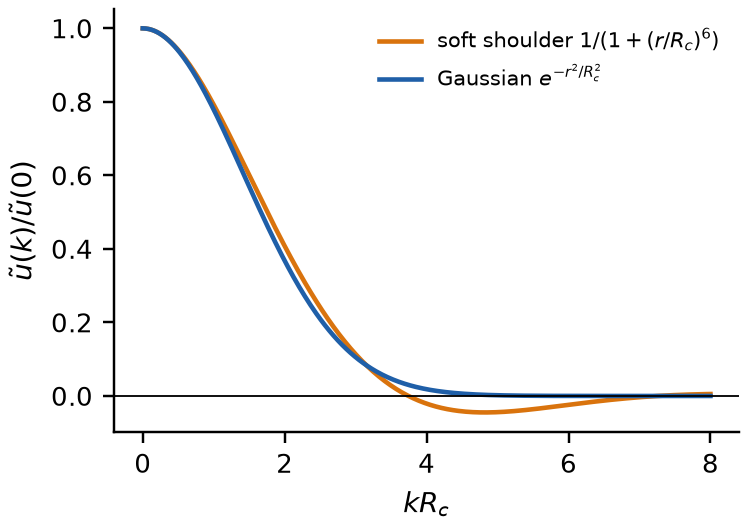
\includegraphics[width=0.52\textwidth]{fig/fig_ft.png}
\caption{Normalised 2D Fourier transforms: soft shoulder $1/(1+(r/R_c)^6)$ (first negative at $kR_c=\ShoulderZero$) and Gaussian (positive). Tier~X, from the same quadrature that reproduces the Gaussian closed form to $\GaussCtlErr$.}\label{fig:ft}\end{figure}

%=====================================================================
\section{The rusty-SUNDIALS SCHA module}\label{sec:rust}
The SCHA is implemented twice. The Python class \texttt{SCHA} (\texttt{B1/code/b1\_lib.py} in the results tree) was written first; the Rust module \texttt{scha.rs} (307 lines, crate \texttt{qf-yukawa-crystal}) is a second implementation of the same Duffy--Gauss zone rule (four triangles with apex at $\Gamma$); only the real-space dynamical matrix differs. It is exposed as
\texttt{lattice\_phonon scha a x y lam n}. It is commit \texttt{9e85e15b23be0c74a665b6a5b74ec02b0bbffc5f} on branch \texttt{physics/p2-zero-point-optimality-2026-10-25} of rusty-SUNDIALS (not pushed at the time of writing; the commit and the blob hash of \texttt{scha.rs} were read from the git object database). The module has three unit tests (harmonic reference agrees with the Poisson zone rule; small-$\hb$ limit with $\hb^2$ remainder; square lattice rejected and large-$\hb$ breakdown).
At paper stage we reran the crate's tests (\texttt{cargo test --offline --locked --release -p qf-yukawa-crystal}): $\RustPassed$ passed, $\RustFailed$ failed, $\RustIgnored$ ignored (\texttt{ledger/rust\_test.log}), and cross-checked Python against the Rust binary on $\CrossN$ shapes: maximum $|E_{\rm py}-E_{\rm rust}|=\CrossMax$ (\texttt{data/crosscheck.json}; e.g.\ $E_{\rm SCHA}(a=1,\rho,\hb=0.1)=0.2267498988201642$ in both).
Clippy and formatting results quoted by the producer were not rerun. This is an improvement in that the SCHA verdict no longer depends on one code, but both codes encode the same equations (Step~7) and the same zone rule: agreement to $\CrossMax$, against a producer $N$-convergence of $3\times10^{-11}$, means identical discrete sums, so it tests the code and not the quadrature, and a common conceptual error would not be caught. The independent-quadrature check is the auditor's midpoint-grid code (Section~\ref{sec:audit}). \tier{X, B1-X-0012}

%=====================================================================
\section{Independent AI audit and revision}\label{sec:audit}
A separate Claude agent audited the first version (\texttt{AUDIT.md}; verdict \emph{ACCEPT\_WITH\_CORRECTIONS}; the physics and mathematics were checked step by step and no change of verdict class was found). It recomputed the headline numbers with code that shares nothing with ours: real-space $D(\mathbf k)$ in fractional coordinates, a uniform half-shifted midpoint grid over the reciprocal cell instead of the Duffy--Gauss rule, a finite-difference Laplacian with Richardson extrapolation, and its own SCHA mixing iteration. Table~\ref{tab:audit} gives its values at $a=1$, quoted from \texttt{AUDIT.md} (not recomputed by us); the SCHA verdict at $a=1$, $\hb=0.15$ is reproduced with a different quadrature and code. This is an AI check, not a human audit.
\begin{table}[t]\centering\small\setlength{\tabcolsep}{5pt}
\caption{Auditor's independent recomputation at $a=1$ (quoted from \texttt{AUDIT.md}, \S1) against this paper's values.}\label{tab:audit}
\begin{tabular}{lrr}\toprule quantity & auditor & paper / data\\\midrule
$\Lap\Est(\rho)$ & $0.4765235166$ & $0.4765235167$\\
$c_{\rm st}$ & $0.119131$ & $0.11913$\\
$\Ezp(\rho)$ ($n=256$) & $1.5033523636$ & $1.5033523522$\\
$c_{\rm zp}$ & $-0.961984$ & $-0.96198$\\
$\hb^*=-c_{\rm st}/c_{\rm zp}$ & $0.123839$ & $0.1238$\\
$\gamma(\hb^*)$ & $0.3130$ & $0.313$\\
$E_{\rm SCHA}(\rho,\hb=0.1)$ ($n=64\to128$) & $0.2267499684\to0.2267499075$ & $0.2267498988$\\
$\Lap E_{\rm SCHA}(\rho,\hb=0.15)$ & $+0.116975$ & $+0.117$\\
harmonic $\Lap E(\rho,\hb=0.15)$ & $-0.10067$ & $-0.101$\\
SCHA $\Delta E$ of $0.30+0.96i$ at $\hb=\Lambda_1$ & $+1.652\times10^{-3}$ & $+1.651\times10^{-3}$\\
harmonic $\Delta E$ of $0.30+0.96i$ at $\hb=0.10$ & $-2.858\times10^{-4}$ & $-2.86\times10^{-4}$\\
\bottomrule\end{tabular}\end{table}
The four blocking items were: (B1) the definition of $a_L$ is in the Astrakharchik et al.\ source (restored, Section~\ref{sec:lind}, ledger row B1-C-0116); (B2) the first version said the negative verdict does not rest on SCHA alone; that is false where $\Lambda_1$ is inside the Lindemann band, and the spinodal reading depends on $\gamma_c$ (corrected throughout); (B3) the title and abstract are rescoped to ``within the self-consistent harmonic approximation''; (B4) this audit disclosure. The nonblocking items are listed with their disposition in \texttt{REVISION.md}.

%=====================================================================
\section{Verdict against the preregistration}\label{sec:verdict}
\begin{center}\small\begin{tabular}{p{0.2\textwidth}p{0.1\textwidth}p{0.6\textwidth}}\toprule item & prior & outcome\\\midrule
B1a harmonic $\hb^*(a)$ & $0.85$ & Confirmed (X). Spinodal exists on $(\RootOne,\RootTwo)$, transition first order, winner on the harmonic stability edge.\\
B1b before melting & $0.4$ & Not supported (X): $\hb^*$ at or beyond the Lindemann band for all $a$ if $\gamma_c\le0.28$ (below the harmonic $0.30$ for $a=\BCBelowALo$--$\BCBelowAHi$); $\Lambda_1\le\Lambda_L(\gamma_c)$ only for $\gamma_c\ge\gamma(\Lambda_1)$ and $a\approx0.5$--$1$.\\
B1c survives beyond harmonic & $0.25$ & Refuted within SCHA (X): none of the sampled stable lattices is below triangular up to $\hb\approx0.27$--$0.33$ ($\gamma_{\rm SCHA}\ge\SchaGammaLowAll$); PIMC blocked.\\
B1d relevance & -- & Rydberg dressing is a soft shoulder (C, quote); no cluster preemption for a pure Gaussian; that quantum melting preempts is our Tier~X inference.\\\bottomrule\end{tabular}\end{center}
\textbf{The kill criterion is met} (\tier{X, B1-X-0013}): the transition ``disappears beyond harmonic'' (SCHA), and the harmonic spinodal lies at or beyond melting for $\gamma_c\le0.28$; the first-order point lies beyond melting except in a window of $a$ and $\gamma_c$, and there the negative verdict rests on SCHA alone. The harmonic prediction does not translate into a structural transition within the only anharmonic theory we could run (SCHA, which omits the second-order cubic $O(\hbar^2)$ term and exchange); this is not a statement that the transition is physically absent.

%=====================================================================
\section{Limitations}\label{sec:limits}
\begin{itemize}\setlength\itemsep{1pt}
\item \textbf{SCHA is not exact} \tier{C, B1-C-0006}. It is a Gaussian variational theory and, for each shape, a Rayleigh--Ritz upper bound on the true ground-state energy. Differences of upper bounds do not order the true energies, so ``SCHA removes the transition'' is a statement about the approximate landscape. Its $O(\hb^2)$ energy contains the quartic anharmonicity at first order but not the second-order cubic term, and the SCHA stiffening we find is itself an $O(\hb^2)$ effect (coefficient $\approx15$--$\SlopeQuadCoef$ at $a=1$, and the fitted $\hb^3$ term is comparable at $\hb\approx0.1$), exactly the order at which SCHA is incomplete; no perturbative $O(\hb^2)$ argument settles the question. It describes neither exchange nor melting. Hence B1c holds within SCHA, and in the window where $\Lambda_1$ is inside the Lindemann band ($a=\BBInsideNarrow$ for $\gamma_c\le0.28$, $a=\BBInsideWide$ for $0.30$), the net negative verdict rests on SCHA alone.
\item \textbf{Lindemann is a heuristic}, $\gamma_c$ carries the $\gamma_c^2$ sensitivity of Step~6, the QMC anchors are for other potentials, and our reading of $\langle(r-r_c)^2\rangle$ as the total 2D displacement is a reading, not a quoted definition (Section~\ref{sec:lind}).
\item \textbf{Only Bravais lattices} with one particle per cell: non-Bravais, striped, cluster or liquid phases are not part of the energy comparison. The competitors are held in shape by an imposed constraint (they are not stress-free), and the harmonic $\Lambda_1$ winners sit on the harmonic stability edge, so harmonic theory does not identify the phase beyond $\Lambda_1$.
\item \textbf{Finite sampling.} $\Lambda_1$ is a minimum over a $0.005$ grid with a stability screen on $48^2$ nodes plus long-wave directions; the best $12$ shapes were re-verified. A coarser stability screen or a finer search could move $\Lambda_1$.
\item \textbf{PIMC not run}; exchange is absent from SCHA. \textbf{Audit}: an independent AI audit (\texttt{AUDIT.md}, ACCEPT\_WITH\_CORRECTIONS, corrections applied) but no human audit; the same pipeline wrote the code, the numbers and this text. \textbf{Literature:} four sources re-read; the rest (\sub) is unchecked; Likos \emph{et al.}\ (cluster criterion) was not opened.
\item Statements about the harmonic functional (P2) are Tier~X there as well; nothing in this paper is formally verified.
\end{itemize}

%=====================================================================
\section{Reproducibility and ledger}\label{sec:ledger}
\textbf{Inputs.} Results copied from \texttt{results/proposal2/2026-10-26/B1/} into \texttt{data/} (\texttt{copy\_data.py}, hashes in \texttt{data/MANIFEST.json}); producer code in \texttt{results/proposal2/2026-10-26/B1/code/} (commands in \texttt{TRANSITION.md}). \textbf{Paper stage:} \texttt{checks.py} (band readings, ray slopes, soft-shoulder transform, Rydberg arithmetic) $\to$ \texttt{data/extra\_checks.json};
\texttt{gen\_inputs.py} writes \texttt{gen\_numbers.tex} and \texttt{gen/*.tex}, from which the tables and headline numbers are generated (a few values are quoted from the producer's record or derived inline, and are marked where they appear); \texttt{make\_figures.py} writes \texttt{fig/}; \texttt{ledger/run\_citation.py}, \texttt{ledger/scha\_crosscheck.py}, \texttt{ledger/verify\_refs.py}; \texttt{ledger/build\_ledger.py} and \texttt{ledger/run\_gate.py}; \texttt{build\_pdf.py}. Python through the repository venv with \texttt{-I}. \textbf{Producer record:} \texttt{data/TRANSITION.md} is an unchanged copy of the producer's file and contains three slips found by the audit (the $2.6\times10^{-5}$ labelled the harmonic $\Lambda_1$ winner is the arc point nearest $\rho$, the winner being $+\SchaEdgeWinOne$; ``dressed-state lifetime $\approx27~\mu$s'' should read bare Rydberg lifetime $27~\mu$s and dressed loss time $130(20)~\mu$s; $100.5$ Hz should be $100.7$ Hz); the erratum is in \texttt{REVISION.md}, and this paper uses the corrected values.
\textbf{Gate.} The Elenchus ledger gate (\texttt{tools/ledger.py}, with the evidence directory) is run on \texttt{ledger/ledger.json}; its verbatim output and exit code are in \texttt{ledger/gate\_output.txt}: exit code 0; 0 blocking finding(s) and 0 flag(s) (the gate's own report; a clean run means the bookkeeping holds, not that any claim is true).

\begin{table}[t]\centering\scriptsize\setlength{\tabcolsep}{3pt}
\caption{Ledger rows (all Tier~C or X; Tier~C rows depend only on Tier~C rows, Tier~X rows on C or X rows).}\label{tab:ledger}
\begin{tabular}{@{}p{0.11\textwidth}p{0.04\textwidth}p{0.80\textwidth}@{}}\toprule id & tier & claim (abridged)\\\midrule\tabinput{gen/tab_ledger.tex}\bottomrule\end{tabular}\end{table}

%=====================================================================
\begin{thebibliography}{99}\small\setlength\itemsep{1pt}
\bibitem{p2} X.~Callens, \emph{Does the triangular lattice minimise the harmonic zero-point energy? A numerical counterexample for completely monotone potentials, with kernel-checked curvature identities}, preprint v1, Zenodo, doi:10.5281/zenodo.23653833 (2026).
\bibitem{textbook} X.~Callens, \emph{The Triangular Lattice and Universal Optimality: human proofs, Lean 4 verification, numerical validation in Python and Rust, and physics from fluids to plasmas (a textbook for students)}, Zenodo, doi:10.5281/zenodo.23295142 (2026); section on quantum melting (Lindemann conventions).
\bibitem{astra} G.~E. Astrakharchik, J.~Boronat, I.~L. Kurbakov, Yu.~E. Lozovik, Quantum phase transition in a two-dimensional system of dipoles, Phys.\ Rev.\ Lett.\ \textbf{98}, 060405 (2007); arXiv:cond-mat/0608246v2. (read, quoted)
\bibitem{prest18} S.~Prestipino, A.~Sergi, E.~Bruno, Freezing of soft-core bosons at zero temperature: a variational theory, Phys.\ Rev.\ B \textbf{98}, 104104 (2018); arXiv:1809.07515v1. (read, quoted)
\bibitem{henkel} N.~Henkel, R.~Nath, T.~Pohl, Three-dimensional roton excitations and supersolid formation in Rydberg-excited Bose--Einstein condensates, Phys.\ Rev.\ Lett.\ \textbf{104}, 195302 (2010); arXiv:1001.3250v2. (read, quoted)
\bibitem{zeiher} J.~Zeiher, R.~van Bijnen, P.~Schau\ss, S.~Hild, J.-y.~Choi, T.~Pohl, I.~Bloch, C.~Gross, Many-body interferometry of a Rydberg-dressed spin lattice, arXiv:1602.06313v3, doi:10.1038/nphys3835 (2016). (read, quoted)
\bibitem{cinti} F.~Cinti, M.~Boninsegni, T.~Pohl, Exchange-induced crystallization of soft core bosons, New J.\ Phys.\ \textbf{16}, 033038 (2014); arXiv:1402.0840. \sub
\bibitem{bonin} M.~Boninsegni, Supersolid phases of cold atom assemblies, J.\ Low Temp.\ Phys.\ \textbf{168}, 137 (2012); arXiv:1201.0980. \sub
\bibitem{mendoza21} A.~Mendoza-Coto, R.~Cenci, G.~Pupillo, R.~D\'iaz-M\'endez, E.~Babaev, Cluster self-assembly condition for arbitrary interaction potentials, Soft Matter \textbf{17}, 915 (2021); arXiv:2010.04631. \sub
\bibitem{prest11} S.~Prestipino, F.~Saija, P.~V. Giaquinta, Hexatic phase in the two-dimensional Gaussian-core model, Phys.\ Rev.\ Lett.\ \textbf{106}, 235701 (2011); arXiv:1107.0828. \sub
\bibitem{mendoza24} A.~Mendoza-Coto, V.~Mattiello, R.~Cenci, N.~Defenu, L.~Nicolao, Melting of the two-dimensional solid phase in the Gaussian-core model, Phys.\ Rev.\ B \textbf{109}, 064101 (2024); arXiv:2209.02802. \sub
\end{thebibliography}
\end{document}
